% Figure -- deterministic (ODE) sampling over training, baseline vs best
% variant per regime. \input{} from Ch6 sec:proteina-anatomy. Replaces the
% all-variant 700K ODE snapshot (now Appendix Table~\ref{tab:proteina-ode}).
\begin{figure}[tbp]
\centering
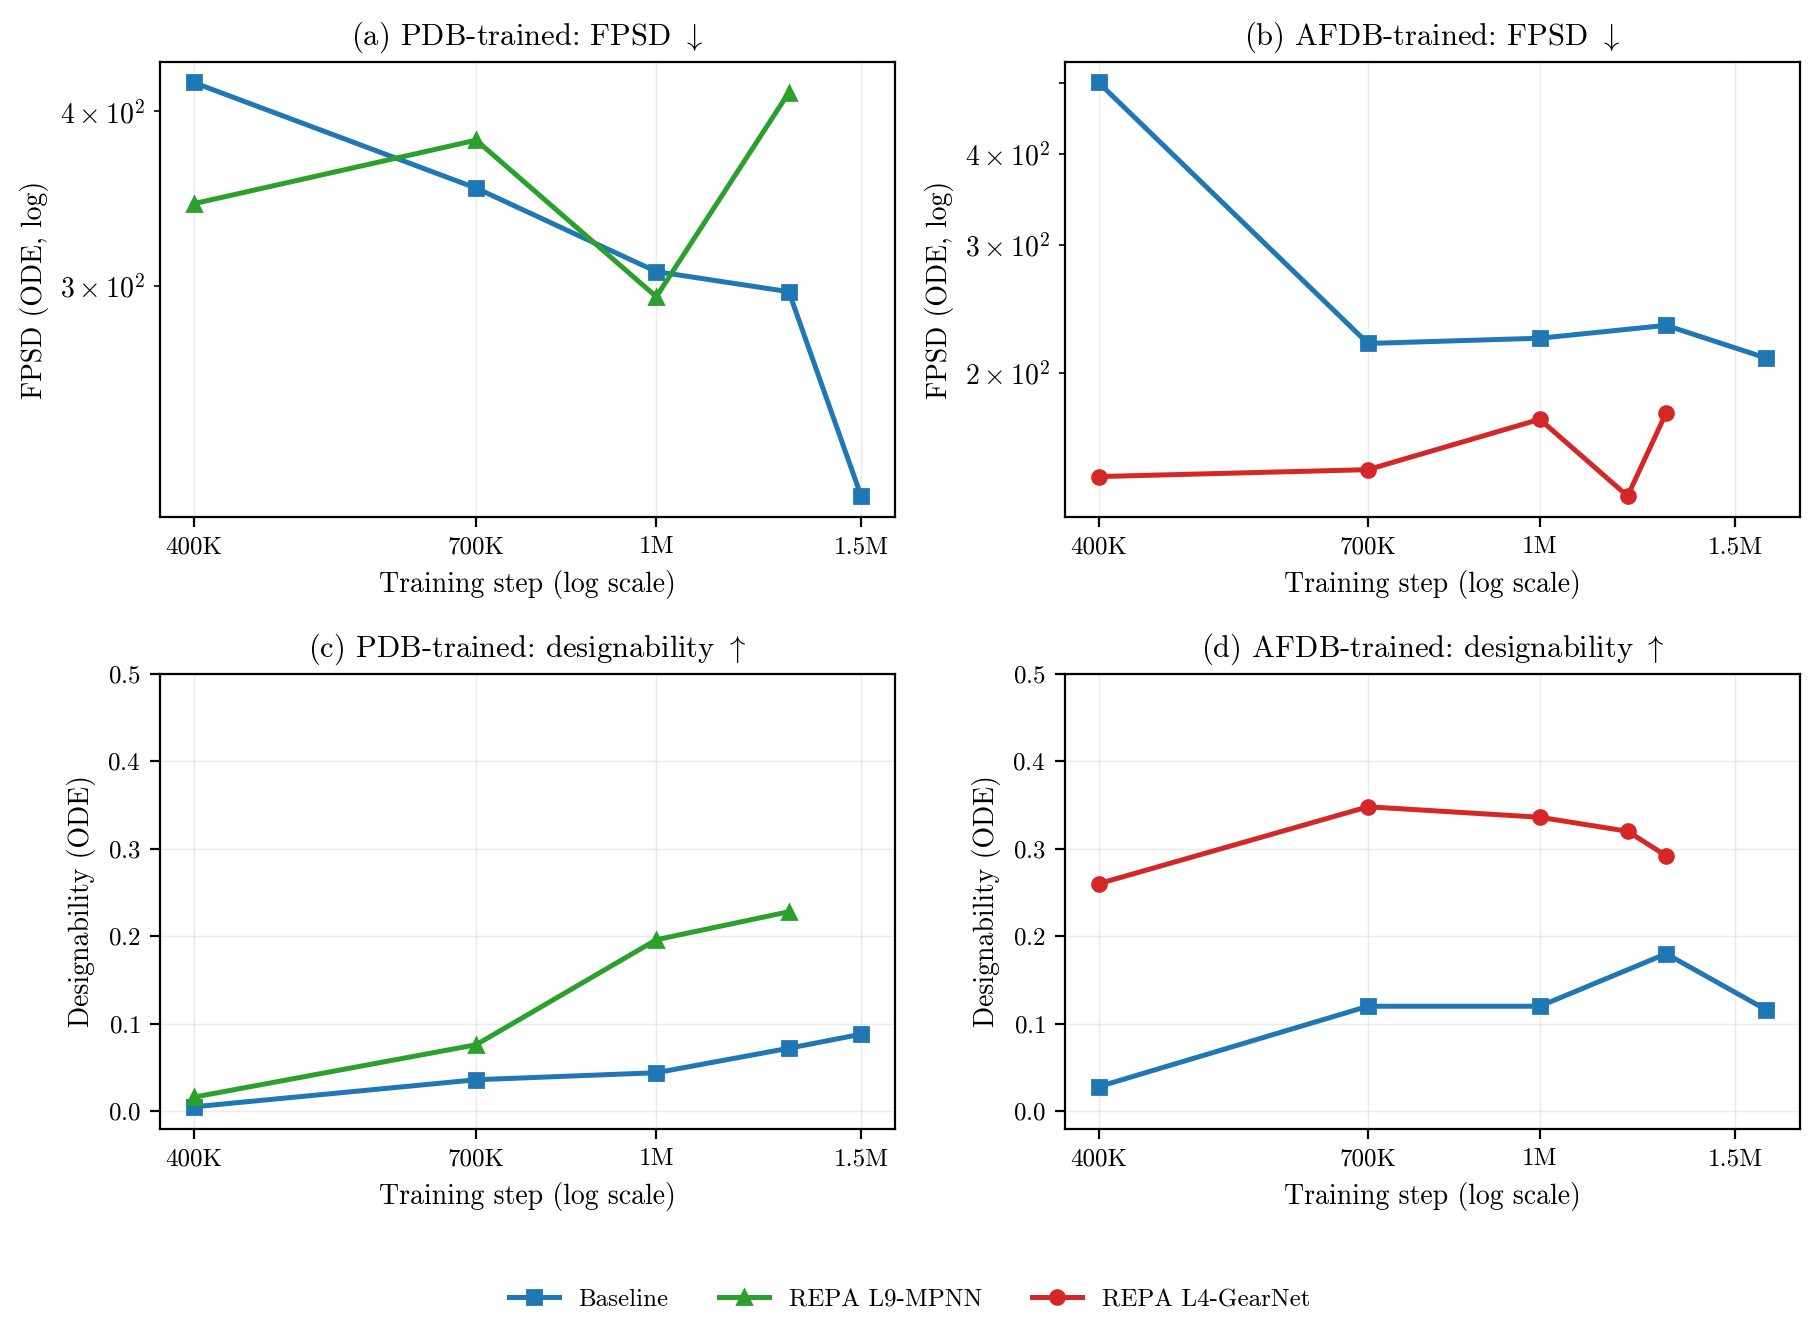
\includegraphics[width=\textwidth]{figures/fig6_ode_trajectory.png}
\caption{\textbf{Under deterministic (ODE) sampling, the AFDB model is genuinely better, while the PDB model redistributes.} ODE sampling integrates the learned velocity field with no injected noise, so it reads what the trunk has learned rather than what the sampler recovers. We follow the baseline and the strongest variant per regime. \emph{AFDB} (right): REPA-L4-GearNet beats the baseline on \emph{both} FPSD (b) and designability (d), across training --- a genuinely better learned field. \emph{PDB} (left): REPA-L9-MPNN wins designability (c) but loses FPSD late (a), so it learns a more designable but less distribution-faithful field. The full all-variant ODE picture at 700K is in Appendix~\ref{app:ode} (Table~\ref{tab:proteina-ode}). (Single-seed; read direction and persistence, not precise magnitudes. From 400K, since earlier checkpoints are barely trained.)}
\label{fig:proteina-ode-trajectory}
\end{figure}
